\documentclass{thesis}

% Better captions:
\usepackage[font=small,labelfont=bf]{caption}
% Sideways stuff
\usepackage{rotating}

% hier namen etc. einsetzen
\fullname{Tamino PSM Hartmann}
\email{tamino.hartmann@uni-ulm.de}
\headline{Implementation of a Java Framework\\ for Marker Based Detection\\ in Augmented Reality}
\titel{Thema}
\jahr{2013}
\matnr{722891}
\gutachterA{Gutachter 1}
\betreuer{Marc Schickler}
\typ{Bachelor thesis }
\fakultaet{Engineering and Computer Science}
\institut{Institute of Databases and Information Systems}

\license{
This work is licensed under the Creative Commons.
Attribution-NonCommercial-ShareAlike 3.0 License. To view a copy of this
license, visit http://creativecommons.org/licenses/by-nc-sa/3.0/de/ or send a
letter to Creative Commons, 543 Howard Street, 5th Floor, San Francisco,
California, 94105, USA. \\ Satz: PDF-\LaTeXe
}

\hypersetup{%
	pdftitle=\pdfescapestring{\thetitel},
	pdfauthor={\thefullname},
 	pdfsubject={\thetyp},
}

% hyphenations:
\hyphenation{Ta-mi-no}
\hyphenation{Hart-mann}

\begin{document}
\frontmatter
\maketitle
\clearpage
\impressum

\cleardoublepage
\setstretch{1.4}

\section*{Abstract}

Due to the drastic increase in powerful hardware in mobile devices, it has become possible to move Augmented Reality applications from desktop systems to their mobile counterparts, thus also opening a wide range of new uses and possibilities.
To allow fast development of mobile Augmented Reality applications, we propose and implement a framework that handles the heavy lifting.

This paper describes the path from design to implementation of an augmented reality framework for the mobile Android platform.
The goal is a framework for marker-based tracking and corresponding rendering of three dimensional objects, to be usable in any application for Android.
The framework, called Imagine, will utilize OpenCV for Android for the image processing to detect markers and OpenGL ES 2.0 to render the corresponding 3D objects.
The finished framework is also analyzed for possible improvements and corrections.

\cleardoublepage
\section*{Gratitude}

The author of this paper would first and foremost thank his social support network in keeping him on track and motivated.
This especially includes his parents for proof-reading the text of this paper, his friends for continually reminding him that a deadline was approaching, and his supervisor Marc Schickler for being great to work with.

Further thanks are due to the online developer communities surrounding OpenGL ES, Android, and OpenCV for explanations and examples.
Thanks are also due to Linux in general for offering a sane development environment, IntelliJ IDEA for a superior and not frustrating IDE compared to Eclipse, and Texmaker for easy \LaTeX .

TODO: Still missing some people! Also, make it sound less cheesy!!!

TAMINO TODO: Where do I mention the programs I used beyond the basic libraries I utilized?


\tableofcontents

\mainmatter
% Overview section
\chapter{Overview}
\section{Introduction}

As mobile devices become more and more powerful and ubiquitous, developers continually realize new uses for them.
One of the fields that is continually reinventing itself is the field of Augmented Reality.
It is the integration of information onto and into our perception of the real world – an augmentation of our reality.
To achieve this many different methods exist.
Many such applications use the user's global position to overlay points of interest onto a camera feed; others use computer vision to track real world objects to enable software interaction with them.
Detecting real world objects is however a non-trivial task, and thus a wide range of possibilities for accomplishing that exist.

One of these is the usage of so-called markers – visually significant patters – to enable fast and easy detection of objects.
To enable quick and easy development of applications that use marker-based tracking for the augmentation of our reality, this paper and the work it covers was envisioned.

This paper represents the initial design and development work for an Android framework to simplify the detection and usage of markers in Augmented Reality applications.
The framework shall henceforth be named \textit{Imagine} to differentiate it from other similar frameworks and the libraries it utilizes.

Imagine will initially only target applications written for Android using Java \cite{android}.
It will utilize the OpenCV for Android library, a sub-project of the original OpenCV framework specifically targeted for Android devices \cite{opencvandroid}.
By separating the detection and the rendering modules within Imagine, it should be relatively easy to extend the functionality of Imagine to other platforms and other technologies, such as desktop applications for Linux or rendering with DirectX instead of OpenGL ES.

To develop and test the framework, we will also implement an application that relies on Imagine for basic functionality.
The application will allow for the real-time viewing of virtual objects on top of a marker and be used to test and evaluate Imagine.
This shall prove the capability and initial concept of the framework and also serve as a starting point for any future derivative work.

This paper consists of all the work done around the actual implementation.
We will look at the basic requirements of the framework.
Basic necessities will be listed and reviewed.
We'll also present a proposal for the structure of the framework.
Difficulties that arose during development will also be documented, along with possible solutions and commentary.
At the end we will also shortly compare Imagine to other frameworks to put it into perspective.

Apart from the programmatic development of the framework and the final review of our work, we will also deliver at least basic documentation for the framework.
For the framework this will include a Javadoc \cite{docjava} file for the completed code and a basic tutorial for usage.
The implementing application should be self explanatory, although care will be taken to ensure a low learning hurdle for using it.

\section{Project Context}

This paper is the bachelor thesis of Tamino Hartmann, written at the Faculty of Engineering and Computer Science \cite{faculty} at the Institute of Databases and Information Systems at the University of Ulm \cite{ulmuni}, Germany.
The work commissioned is to create a framework for fast and easy integration of marker-based tracking for possible future projects within the institute, thus decreasing repetitive re-implementation of the same features and allowing a faster development time for implementing applications.
The supervisor was Marc Schickler and the examiner was Professor Doctor Manfred Reichert.

\section{Content of this Paper}

Chapter \ref{framework} presents the preliminary work done for finding an algorithm and subsequently for implementing it.
We then shortly take a look at what encompasses our markers for Imagine in chapter \ref{section_markers}.

Chapter \ref{results} presents our encountered difficulties, implemented features, and a comparison to other, similar frameworks.
We conclude with chapter \ref{conclusion}, where we step back and give a more general outlook on possible future work.

% Section on the framework
\chapter{Framework}

In this section, we take a close look at the proposed structure and capabilities of the framework, Imagine.
We will then discuss the implementation and its difficulties.

\section{Proposed Functionality}

The framework shall have two primary capabilities: first, it should enable fast and easy access to the 3D pose calculated from the detected marker.
Second, given a digital 3d model to display, it should be capable of returning a rendering of the object within the scene on top of the live preview, correctly positioned.

Generally, the framework shall work as in the following.
Once the framework is running, OpenCV reads the camera frame directly from the camera.
This frame is copied to the worker threads that will detect markers.
The original unaltered frame is passed back up to be shown as the background of the later rendering.

These worker threads are where the computational expensive part of actually detecting the marker happens.
Using the OpenCV for Android library, we detect markers and calculate their three dimensional pose.
All detected markers are put into a list with the important attached information, such as the corresponding identification number of the detected marker.

This list is passed back to the main controlling element of the framework.
Here it can be passed directly to listening classes if that option was chosen.
This is done when only the marker information is required and not a rendering.
If not, the list is filtered for only those markers that the user wants to track.
These trackables have to have been registered beforehand by the user.
Then the model information is attached to all detected trackable assets and passed down to the rendering part of the framework.
Here, this filtered and supplemented list is used to render all objects onto the correct positions with the correct perspective modifications on top of the camera image.

Apart from the above mentioned basic functionality capabilities, the framework should also handle the easy gathering of performance and error information, mainly by extending the relevant functions of Android.
This can include gathering the logs to a listener, bypassing the Android logging mechanism, and any further functionality that could be useful.

\begin{figure}
	\centering
	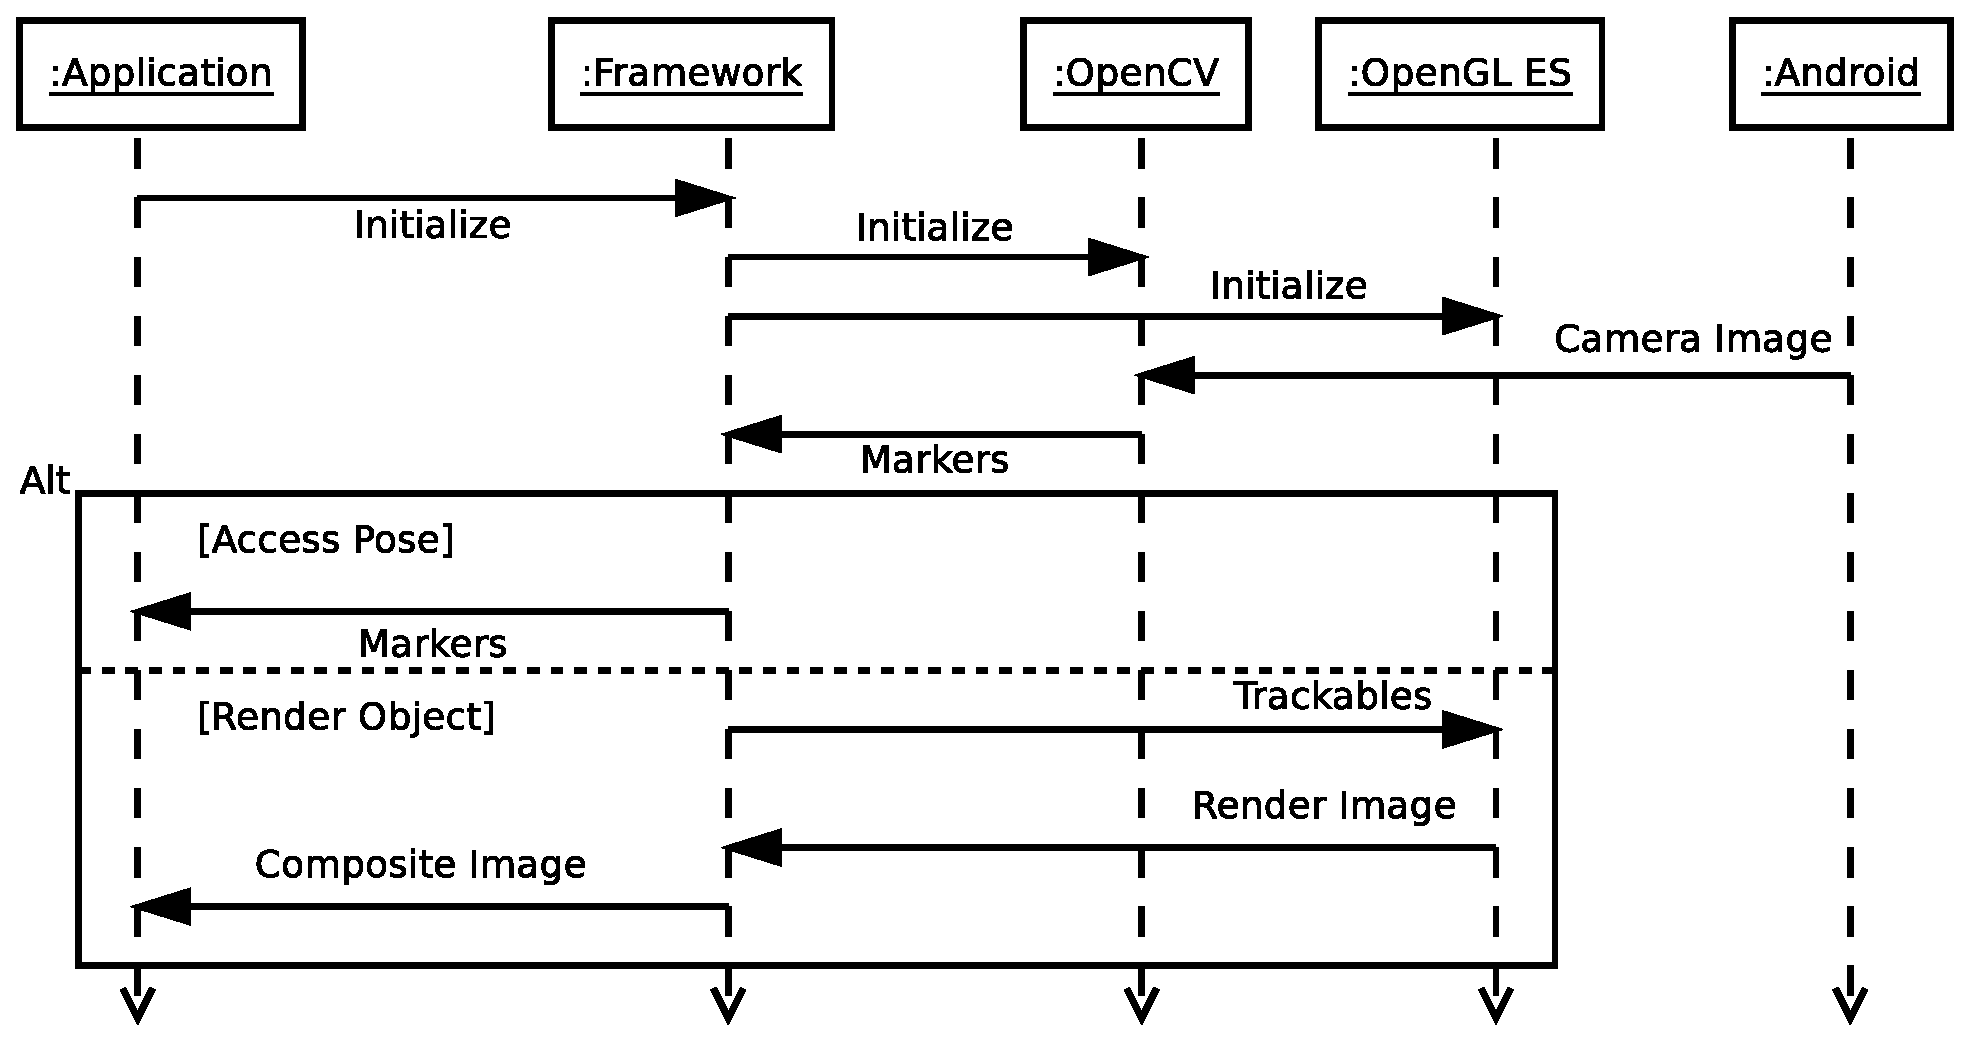
\includegraphics[width=12cm]{img/sequence_access.eps}
	\caption[Access Sequence.]{The proposed sequence of the workflow with the framework, using OpenCV for Android and OpenGL ES.}
	\label{fig:sequence_access}
\end{figure}

Figure \ref{fig:sequence_access} shows the proposed sequence of events of Imagine, and where data can be input or read.
As proposed, the framework should offer a wide variety of uses, without being overly complex from an outside perspective.
Another important aspect we want to make possible is the possibility of changing all the more important parameters during runtime, such as switching the model or adding a new marker.
This should allow a less restrictive usage of the framework and any derived apps as a result.

\section{Dependencies}

Primary dependency is of course an Android environment, given that it is the target platform for the framework.
The framework is written in Java with Android specific syntax and structure.
Aside from the basic requirements, the framework will depend mainly on two external software solutions.

The first is OpenCV\cite{opencv}, an open source collection of computer vision and machine learning software.
Imagine makes use of the Java-based port, called OpenCV for Android.
To use the framework on Android, the OpenCV Manager\cite{opencvmanager} needs to be installed alongside the application using the framework, as the marker detection relies on it.
The OpenCV Manager offers the best version of OpenCV for Android for each Android device according to its specifications and capabilities.

Apart from OpenCV for Android, OpenGL ES is used for the rendering of the 3D objects to the display.
For this dependency, nothing has to be considered from an application that would use the framework, as the mobile version of OpenGL is already built into Android.
According to the capabilities of the developer device used, we choose to use OpenGL ES 2.x.
This has the added advantage that at the time of development, a minority of devices support OpenGL ES 3.x anyway.
At the same time using version (OpenGL ES 1.x) would broaden the pool of compatible devices by an insignificant amount.

\section{Limitations of Scope}
\label{scope_limit}

In the following we will look at the features required of the framework for it to be considered feature complete and basically usable.
Some nice-to-have features will also be listed, meaning features that will not be implemented but could possibly be interesting for future development.
For completeness we will also take a short look at features that are possibly too difficult to do and or would require significant work.

To clarify the scope of the proposed framework, all features that will be delivered are described within the following table:

\begin{tabulary}{\textwidth}{L || L}
Debug messaging & The framework should be easy to debug and allow simple access to status messages\\
\hline
Manage trackers & Allow to add and remove trackers during runtime\\
\hline
Read position data & Give the possibility of accessing the raw data returned from the OpenCV interface, bypassing the rendering step\\
\hline
Configuration & Allow easy visualization for various aspects of the framework\\
\hline
Multi-threading & Allow computationally expensive tasks to run multi-threaded\\
\hline
Helpful functions & Offer functions for marker creation and object loading to decrease external work required to use Imagine\\
\end{tabulary}

The features in the following table are features that could be implemented relatively easily.
Future work should begin with these features to expand the use-cases of the proposed framework.

\begin{tabulary}{\textwidth}{L || L}
Animated Objects & Allow the object to have an animation and offer access to control animation dynamically.\\
\hline
Simple Advanced Rendering & Allow textured rendering and other visual improvements.\\
\end{tabulary}

The following are features that will not be implemented.
These features would possibly require significant work to include and change fundamental parts of how the framework currently runs.

\begin{tabulary}{\textwidth}{L || L}
Marker-less Tracking & Foregoing markers and allowing any feature-rich object to be used instead.\\
\hline
Fancy Rendering & Alternative rendering output, such as stereoscopic output to be used by 3D capable viewing devices.\\
\hline
Occlusion & The capability to detect where scene occlusion is taking place and render accordingly.\\
\hline
Real-time Detection & Raise performance enough to be perceived as smooth, no detection lag.\\
\end{tabulary}

For broader future possibilities concerning the use and further development of Imagine, see also section \ref{future}.

\section{General Class Diagram}

\begin{figure}
	\centering
	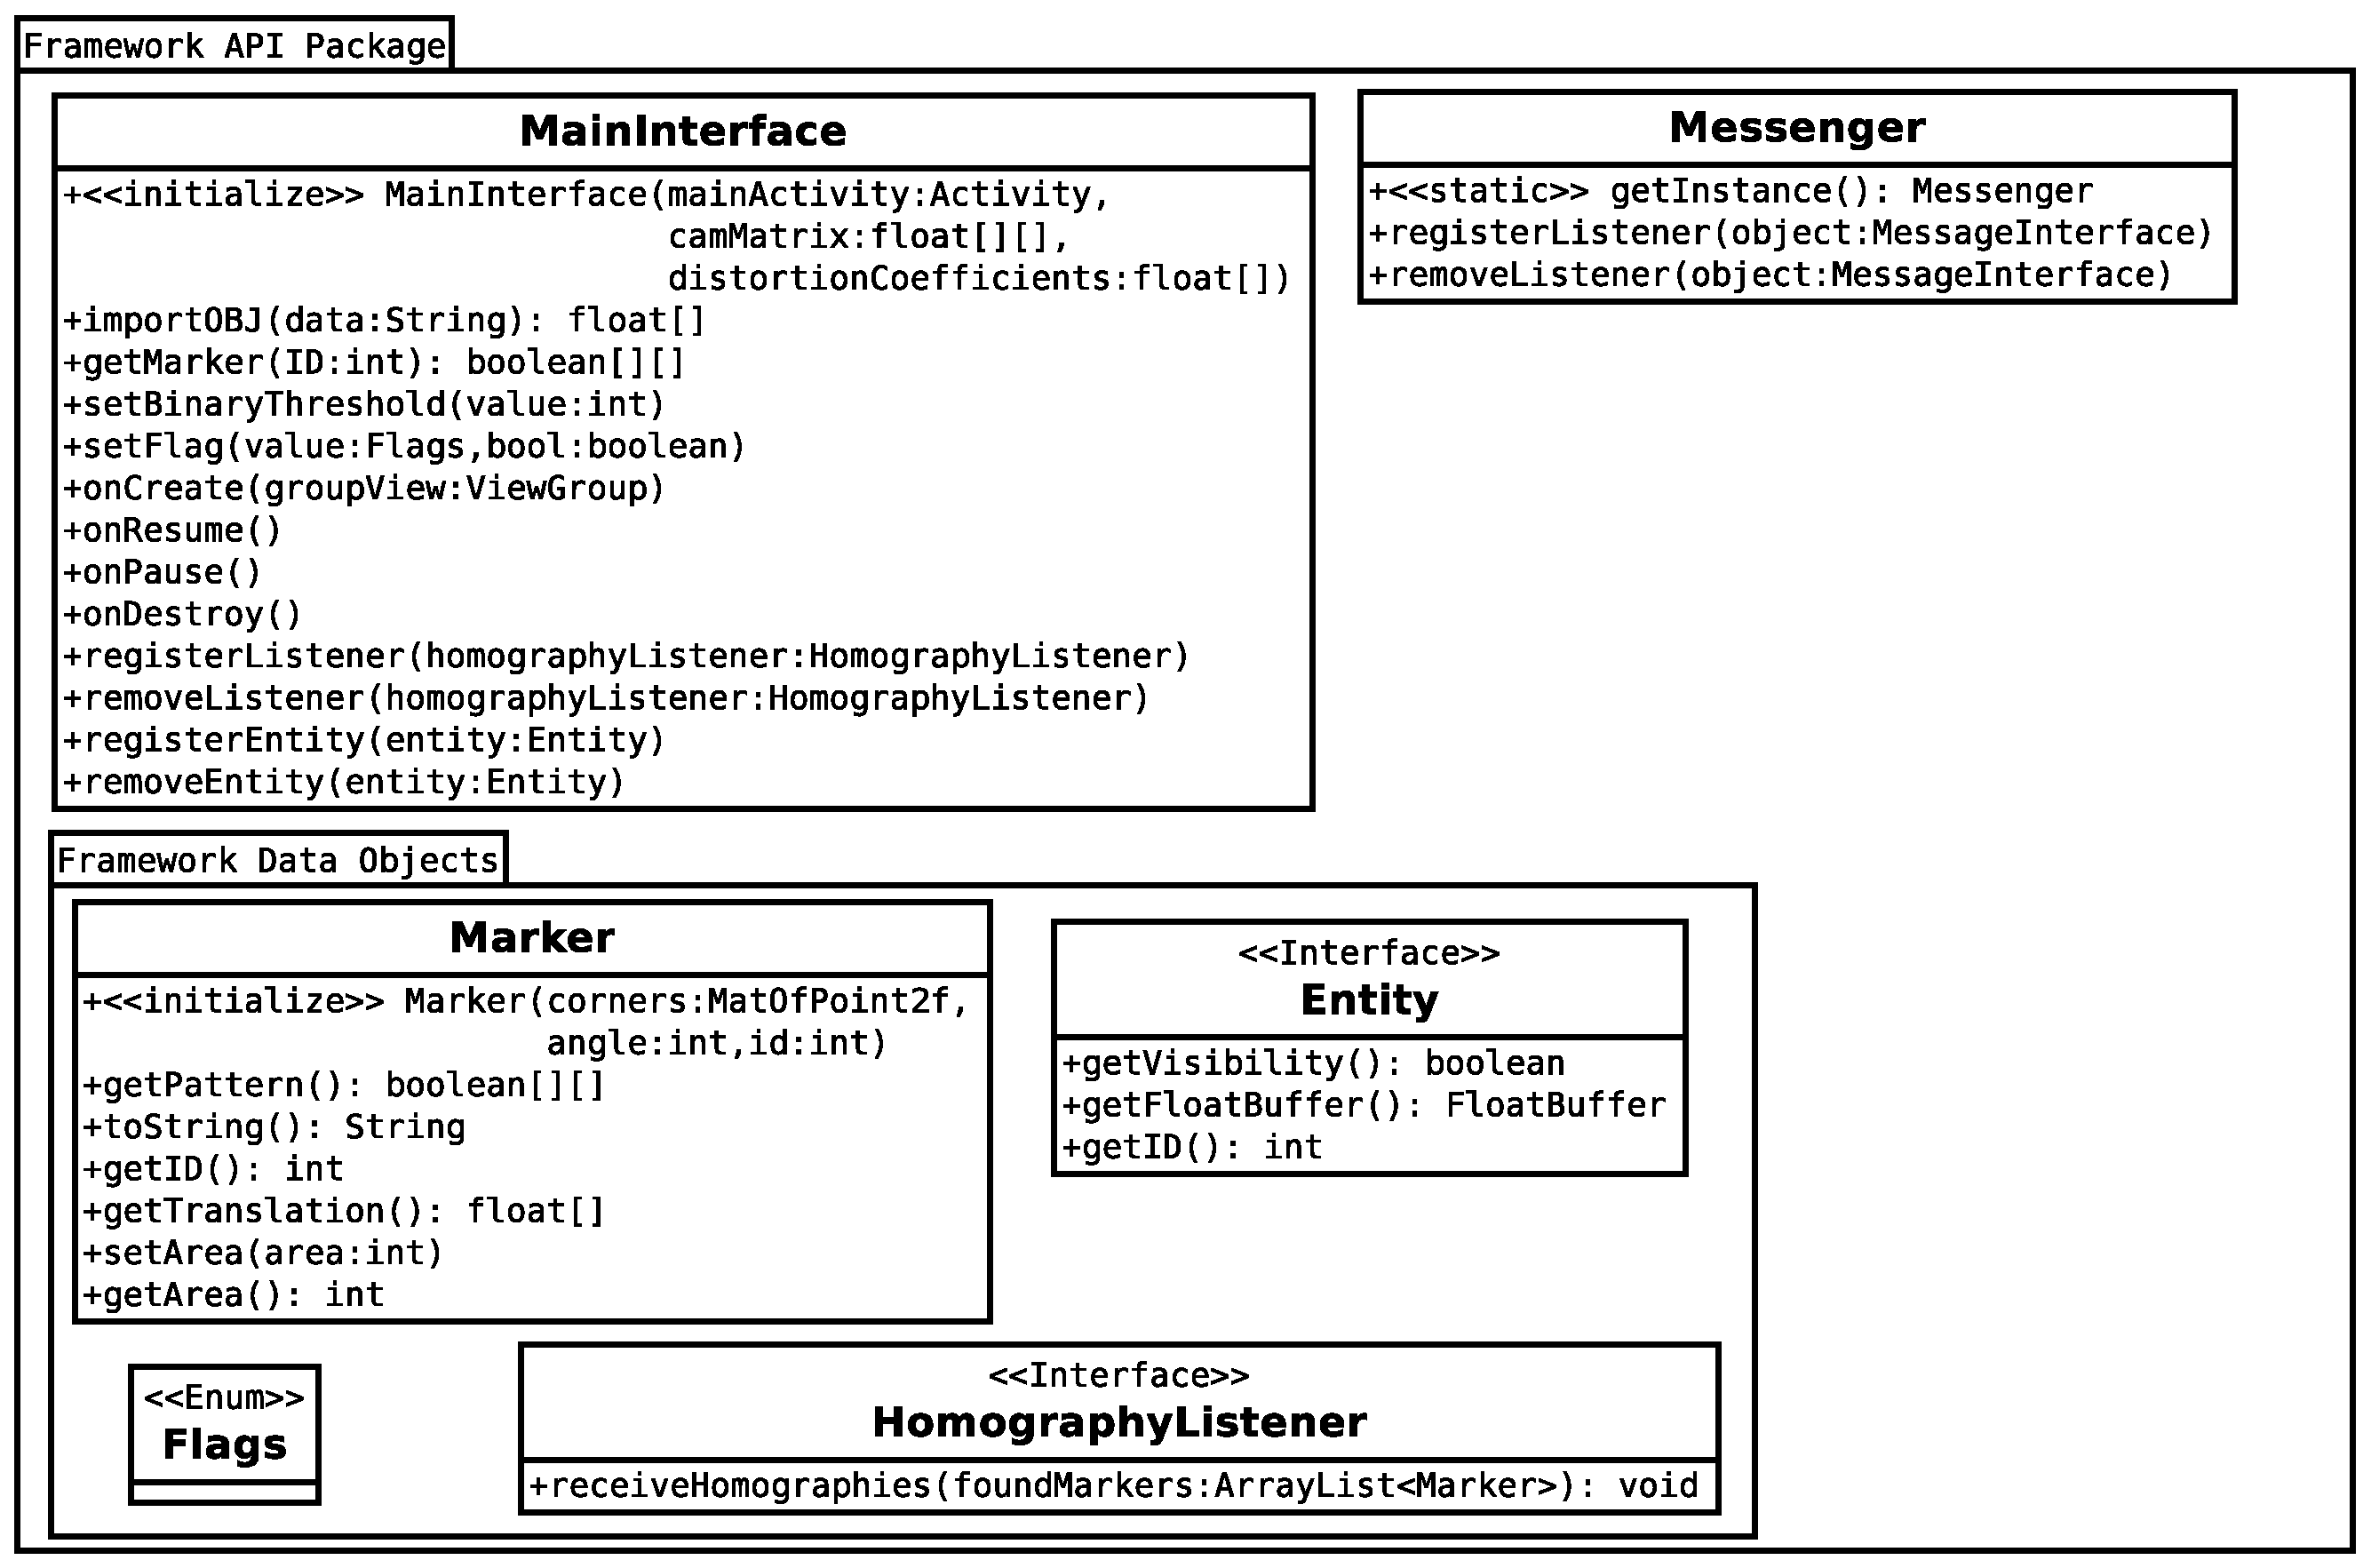
\includegraphics[width=13cm]{img/class_diagram.eps}
	\caption[Public Class Diagram]{This is the preliminary class diagram of the proposed functionality of the framework accessible from outside. It also includes data objects and interfaces required for meshing the application with Imagine.}
	\label{fig:class_diagram}
\end{figure}

Now let us take a look at the proposed class structure of the framework, as illustrated in figure \ref{fig:class_diagram}.
For the complete class diagram, see section \ref{complete_class}.

Main access is controlled over the framework controller, labeled MainInterface, which almost exclusively contains all the public methods callable from outside of the framework that matter for normal usage.
Apart from MainInterace, the log messages can be listened to via the Messenger, ConvertHelper offers Mat and float conversions, and MarkerPatternHelper offers methods for generating and detecting markers.\footnote{TAMINO TODO: See issue tracker on Github, should be consolidated into MainInterface if possible!}

Some data object classes are also accessible as public classes to ease data transfer.
Notably, this includes the Marker class for accessing the pose information and the Flags class for controlling flags for Imagine.
Interface classes are also provided for passing and receiving information.

\section{Application Programming Interface}

The following represents the methods that make up the more important aspects of the framework.
With the listed methods, all functionality that the framework offers can be accessed.

{\footnotesize
\begin{tabulary}{\textwidth}{J || J}
<<Initialization>> & Constructs all the internal classes and prepares the major functionality. Also used to set the most important values such as camera distortion and camera perspective, as these are crucial for a correct processing. Furthermore also used to set the output layout where the results are drawn to.\\
\hline
onCreate & Must be called in the activities onCreate; handles all the necessary calls within the framework.\\
\hline
onResume & Must be called in the activities onResume.\\
\hline
onPause & Must be called in the activities onPause.\\
\hline
onDestroy & Must be called in the activities onDestroy.\\
\hline
registerListener & Add a homography listener. Listeners will be called if the correct flag has been set. Listeners will receive a list of detected markers containing all information.\\
\hline
removeListener & Removes a homography listener. \\
\hline
registerEntity & Adds an entity containing the ID, visibility status, and vertice buffer. This means that upon detection of the corresponding marker, the object will be rendered on top of it, according to the status of the visibility.\\
\hline
removeEntity & Removes an entity from the list.\\
\hline
setDebugFlag & Sets the given debug flag. For possible flags please see the Javadoc.\\
\hline
removeDebugFlag & Unsets the given debug flag.\\
\end{tabulary}
}

Important to note is that the onCreate, onPause, onResume, and onDestroy methods are inherent to the way programs work on Android, and thus must be called for the framework to function correctly.

Upon initialization of the framework, entities can be added to be tracked and rendered with the registerEntity method.
To do that, the user has to implement the entity interface, providing functionality for reading the identification that the object is to be bound to, whether it is to be rendered (the visibility option), and finally a FloatBuffer containing the vertice location and color information.
The use of the FloatBuffer might not seem intuitive at first glance, however it allows the framework to handle the rendering all on its own, greatly simplifying the usage of the framework.

\section{Usage}

The finished framework can track multiple markers in a single instance.
In fact, it tracks all markers it finds from the beginning, only filtering out the ones that the user is interested in before rendering.
This allows comparatively easy use of multiple, separately tracked entities.
However, this also has a significant drawback: as the framework is computationally expensive, multiple markers can quickly degrade its performance, even if the user is only interested in a single marker – see also section \ref{performance}.

For the tracking to work, the marker must be visible to the camera.
The marker can be shown on a separate screen, printed on paper, or drawn.
The framework will then detect the presence of the marker, continue with its identification and perspective information, and finally store it as a successfully detected marker for the render interface to render.
Utilizing the thus calculated perspective information, paired with the correct object, the renderer then proceeds to render objects onto their respective markers.

\section{Implementation}

The following section describes in more detail the implementation of the framework.

\subsection{Tools and Environment}

We developed Imagine on a Linux Mint Debian Edition powered computer with the IntelliJ IDEA IDE\cite{idea}.
The development device was connected via USB debugging for rapid iterative coding.
Javadoc was written directly into the code and then generated to readable format via internal IntelliJ IDEA tools.

For further documentation, we utilized Dia\cite{dia} for generating diagrams, Umbrello\cite{umbrello} for the class diagrams, Texmaker\cite{texmaker} for \LaTeX  creation, and Git\cite{git} for revision control.

Imagine was developed with the target of running smoothly on a Nvidia Tegra 3 processor.
The development device is the Transformer Prime, a 10'' tablet from ASUS\cite{devicedev}.
This means that the framework should run smoothly on a 1.6Ghz Quadcore ARM processor rendering to a 1280 by 800 pixel screen.

\subsection{First Steps and Trials}

First we implemented a test project to experiment with OpenCV for Android to collect data on possible solutions and problems.
This test project was later worked into the finished framework once a suitable algorithm had been found.

At first, a feature-based detection approach for markers was tried.
That meant that feature detection was used on the marker, resulting in a cloud of key feature points.
These can then theoretically be located in an image from which we have likewise extracted feature points.
However, this method proved to be too computationally expensive considering that we would then still need to identify the marker and calculate the geometric information.
Initial tests only for detecting feature points in a live camera view yielded framerates below 2 frames per second.
This was deemed insufficient for a realtime use of the finished product.

Initialized by that, further detailed research turned up a better solution based on the method used by the comparable Aruco\cite{aruco} framework.
By comparing the performance of the marker-based approach of Aruco, the feature-based approach was discarded in favor of a marker-based approach, as it promised to offer a significant performance increase.

\subsection{Implemented Algorithm}
\label{detection_workflow}

This section describes in detail how we detect, identify, and calculate the perspective transformation of the markers in Imagine.
These steps are done for each frame, leveraging the image processing capabilities of OpenCV.
It results in a list of detected markers with their transformation matrices.

The first step is to reduce the color image into a binary image.
To do this, we take the gray-scaled image that we receive from OpenCV and threshold it against a constant value.
As we are interested in highly contrasted regions as our markers are monochrome, this threshold was chosen relatively low.
Alternative methods are available, but either have other drawbacks or take a longer amount of time\footnote{TAMINO TODO: Redo when done, other methods should work now too!}.

This binary image is suitable for fast detection of all contours within the image.
The detected contours are then filtered for size, as any contour that represents a marker below a certain size will be too small to safely and correctly identify.
The filtering also improves performance as it removes much contour noise, therefore decreasing our workload for further steps.
Next we calculate polynomial approximations for all remaining contours.
We can then filter the polynomial objects based on criteria for our markers.
Of these criteria there are two: only objects with four corners and those which form a convex hull are kept.

Now that we have a selection of detected perspective rectangles that might be markers, we sample all candidates for a black border.
To do this, we first have to de-warp the part of the image that is confined by the rectangles.
This is done to decrease sampling difficulty and decreases speed only by an insignificant amount.
The now square texture is then used in the following steps, of which the first is to check that the candidates have a valid black border.
Next we check for the orientation bits: if we find these, we can be comparatively sure that we have a valid marker and can continue to its identification.
If the detection of orientation fails (meaning that we do not find a pattern of three white and one black inner corner block), we consider the candidate to be invalid.
Now all that remains is the marker identification, which is done by sampling the remaining inside bits and decoding them.
This process is further detailed in section \ref{section_markers}.

One of the major advantages of the polynomial representation of the markers is that it is very easy to calculate the 3D position of the markers from them.
This is done by solving a linear equation that tries to find the translation values required to move the marker from the camera plane correctly to its 3D location according to its perspective distorted location.
That step is the one that requires the camera matrix and camera distortion values, which have to be determined beforehand for each device.
The resulting translation is saved along with marker identification and angle.
It will later be used to correctly place an object on top of the marker to be rendered in OpenGL.
All thus detected marker candidates are then passed to the main controller, which manages them for the renderer.

For further commentary on the implementation, see section \ref{implementation}.
Concerning final performance of the framework, see section \ref{performance}.

\section{Complete Class Diagram}
\label{complete_class}

Figure \ref{fig:complete_class_diagram} shows the complete class diagram of the finished framework.

MainInterface encapsulates all the primary functionality within the framework that is required to work with if from an application.
Apart from managing all the other classes on startup and closure, it also handles the information exchange between them and the application itself.
It also enables the management of the entities and their assigned trackables\footnote{TAMINO TODO: Add to glossary!}.
MainInterface also handles any inter-system compatibility that the passage of information between the renderer and interface require, such as the filtering of detected markers for trackables that are to be rendered.

The Messenger class allows easy and quick access to any debugging, logging, or error messages to outside classes via a listener principle.
This allows outside threads to be directly notified when a message is written and allows the end user to expand on any messages from the framework.

The OpenGLRenderer implements the functions that take the list of detected trackables and renders their objects onto the position given by the pose estimation.
This class also implements all functionality for the rendering types and 3D drawing functions that are required.

The OpenCVWorker is a single thread that continually takes an input image and tries to detect all markers in it.
The functionality itself however rests in the Detector class; this class only handles the logical functions surrounding the multithreading and work delegation.

The Detector class is where the main detection code lies.
The algorithm was thus extracted from other classes to allow a clean differentiation in functionality.
Here, the main OpenCV work is done.
Detector also implements a few internal methods for the detection work that would be ill suited to lay elsewhere.

\begin{sidewaysfigure}
	\centering
	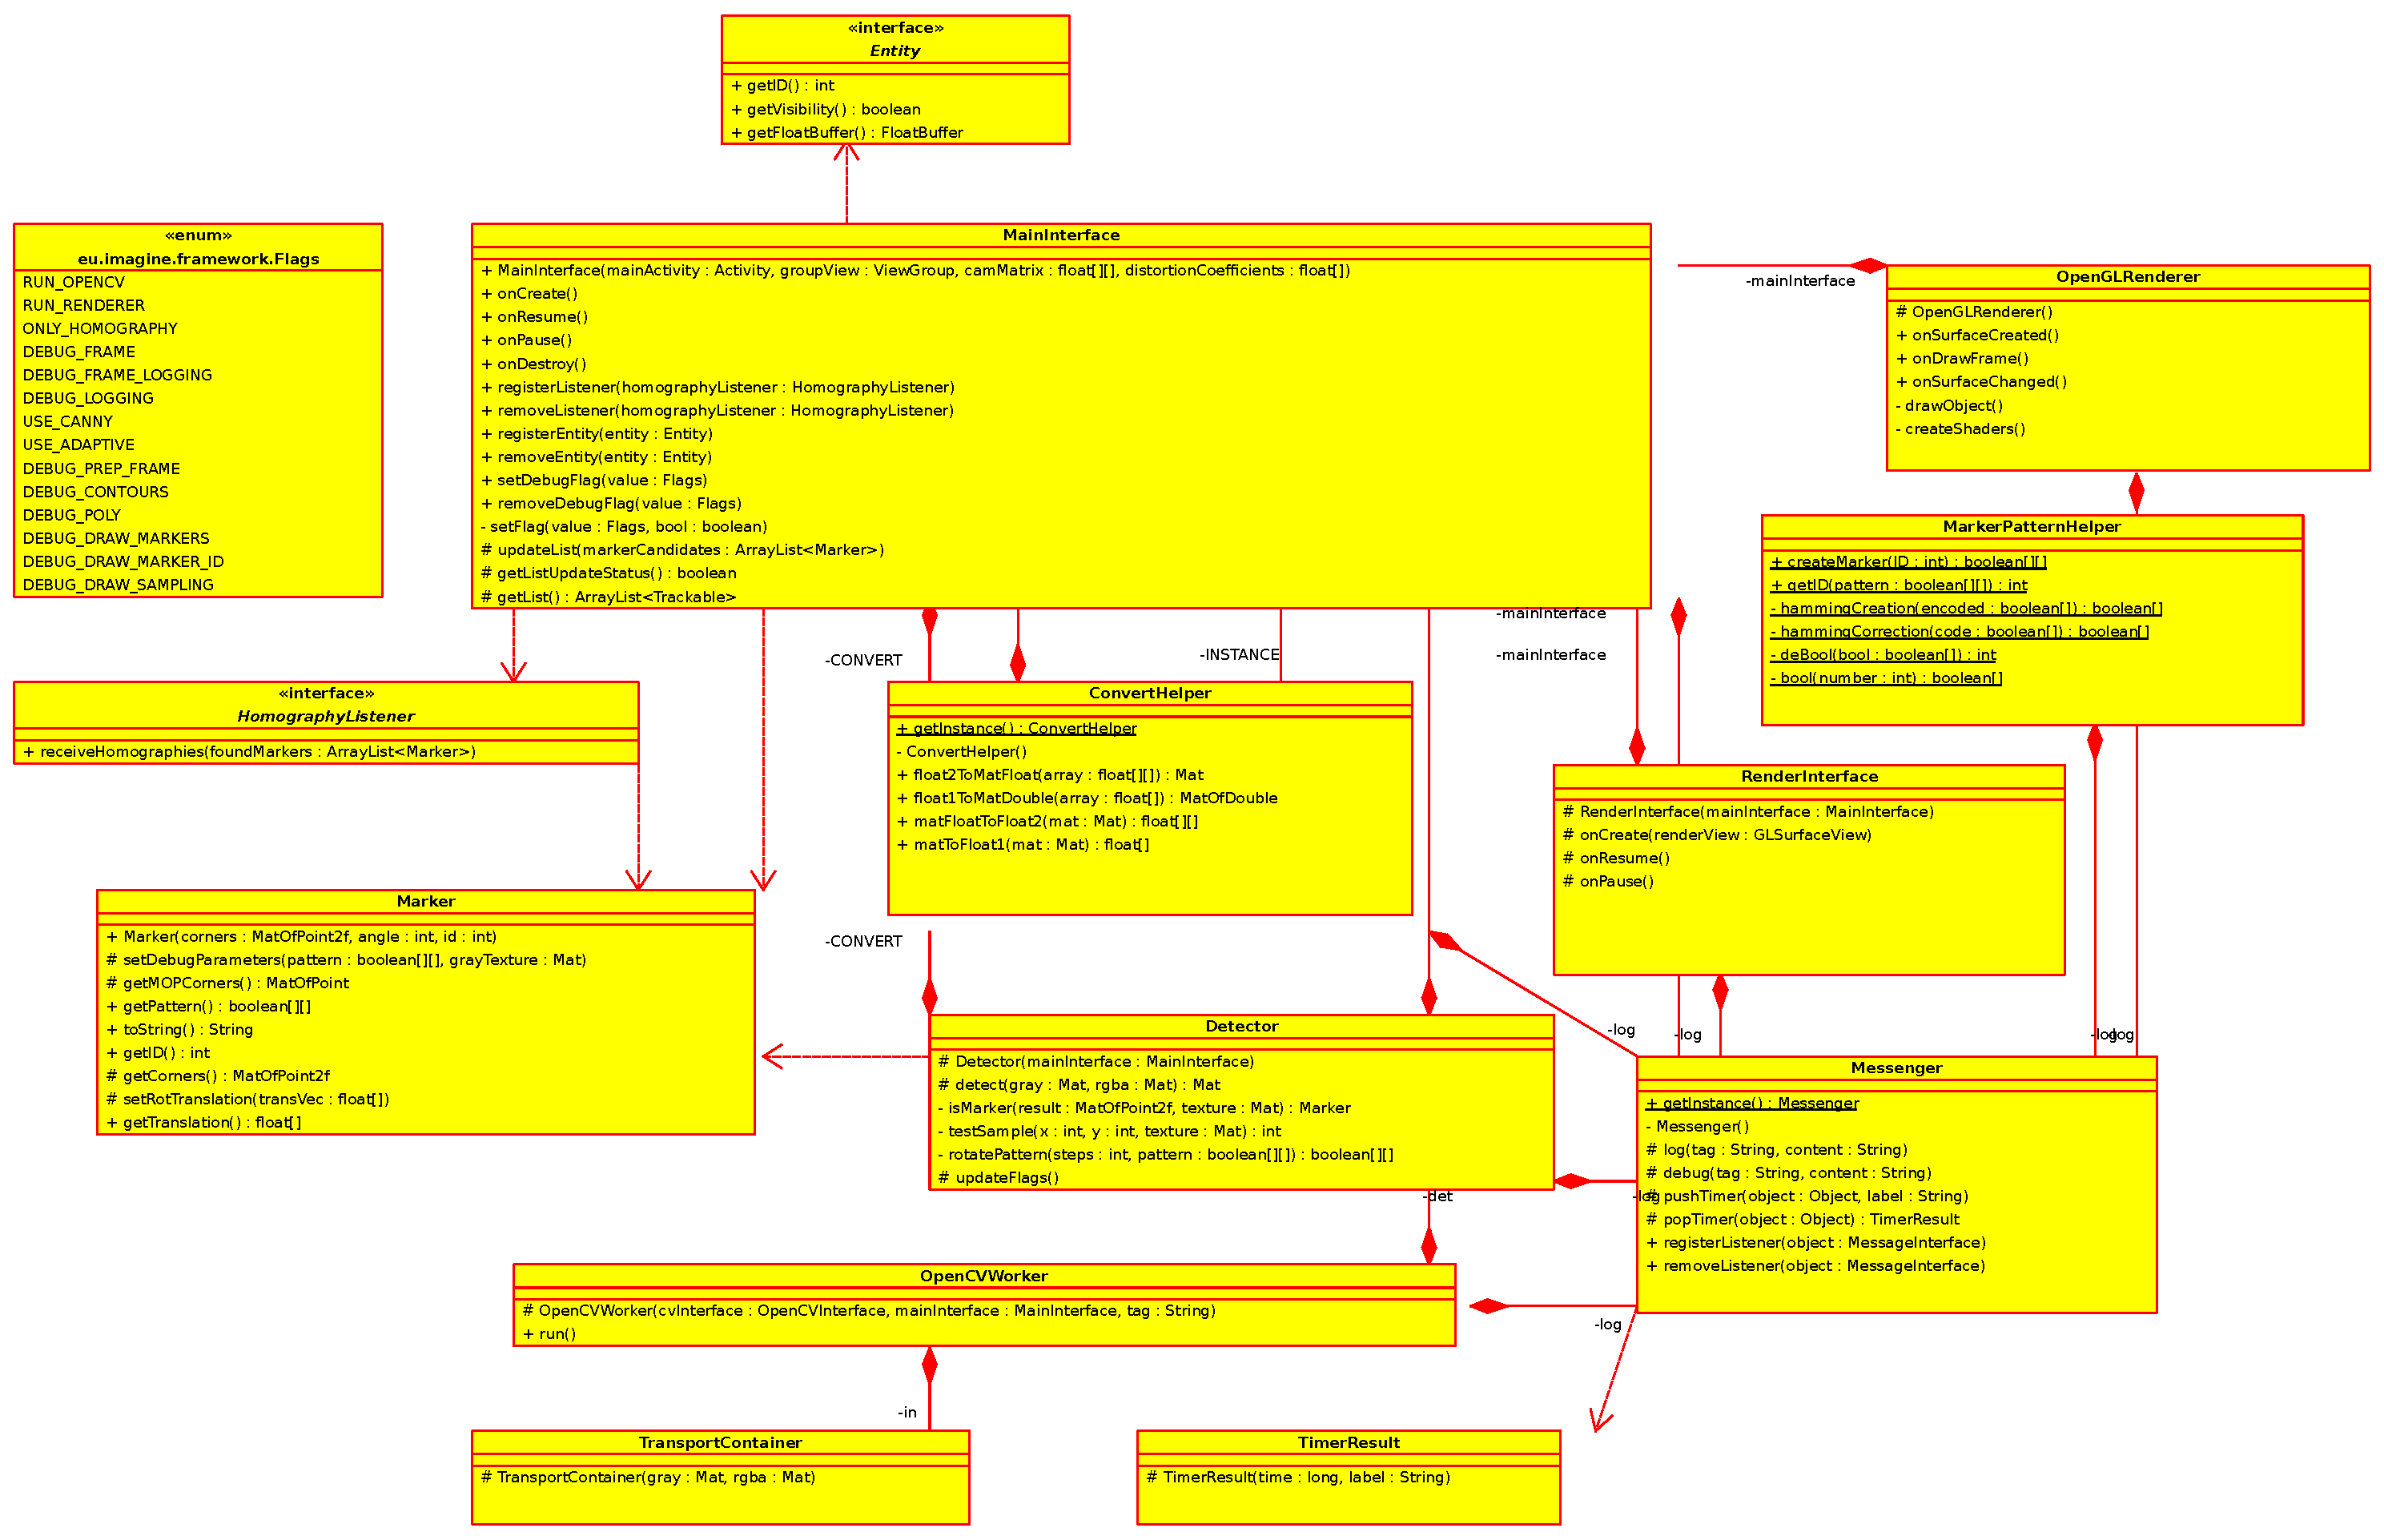
\includegraphics[width=21cm]{img/complete_class_diagram.eps}
	\caption[Complete Class Diagram]{This is the complete class diagram of the Imagine framework. It lists all methods of all the public, protected, and private classes. Attributes were left out for formatting reasons; especially the Detector class has a large amount of attributes that would not fit into this diagram.}
	\label{fig:complete_class_diagram}
\end{sidewaysfigure}

The above proposed system should enable an easily extensible build for the framework while retaining a simplistic use case.
It should, in theory, be relatively easy to exchange either the worker threads or the render class to enable the framework to run beyond Android.
That would enable the framework to run on normal personal computers using the full-fledged version of OpenGL or possibly DirectX.

\section{How to Use}

Using the framework is very easy.
Simply create an instance of the MainInterface of the framework either in the constructor or in the onCreate method of the activity where the application is run from.
After creating the instance, the onCreate method of the framework must be called from within the activity's own onCreate method.
To create the framework, an Android GroupView is required.
Here it will place the camera view and the view responsible for rendering the detected objects. Also required are the camera values for the target device.
These can either be calculated, copied from device information, or detected with an application like the following: \url{https://github.com/Itseez/opencv/tree/master/samples/android/camera-calibration}.
Now all that remains is to also call onPause, onResume, and onDestroy in the respective functions of the activity via the framework.

The framework offers some helper functions to shift some workload away from the user.
These should allow the usage of the framework to be very quick to learn and implement, without having to understand how the framework works internally.

One such helper function is the creation of correct markers in the form of a binary array.
This can be used one-off to create a printable set of markers, or during use of the framework for internal representation of markers.
The method takes the identification number and generates the complete marker for it, including border, orientation bits, and Hamming encoding.

Another helper function loads a 3D model file and converts it to the correct representation to be used with the entity class.
This method takes a 3D model file and converts it to the FloatBuffer data structure used by the framework, if capable.

% Section on Markers
\chapter{Markers}
\label{section_markers}

To enable the framework to detect a 3D pose from a video feed, a marker with specific properties will be required.
A marker is a visually significant pattern that the system can detect within an image and can be used to calculate spatial coordinates.
Figure \ref{fig:marker_example} shows an example of such a marker.

\begin{figure}
	\centering
	
\includegraphics[width=4cm]{img/marker_example.png}
	\caption[Example Marker.]{An example of a marker. This image is either printed or displayed by some other means in the real world to allow a system to use it as a reference to base a virtual overlay off of it.}
	\label{fig:marker_example}
\end{figure}

Due to our approach for marker detection, we selected a square black on white marker.
Other types exist, such as rotary markers or image-based feature markers.

\section{Coding Scheme}

For this framework, a marker is coded as seen in \ref{fig:marker_template}.
The basis is a six by six sized grid, where the border is solid black.
The internal four by four spaces are used to encode the orientation and identification of the marker.
The orientation is encoded by coloring the corners white except for the top right corner, which is encoded black.
The identification is binary encoded with a Hamming code\cite{hamming} for error detection and correction.
Parity bits are the red bits.

\begin{figure}
	\centering
	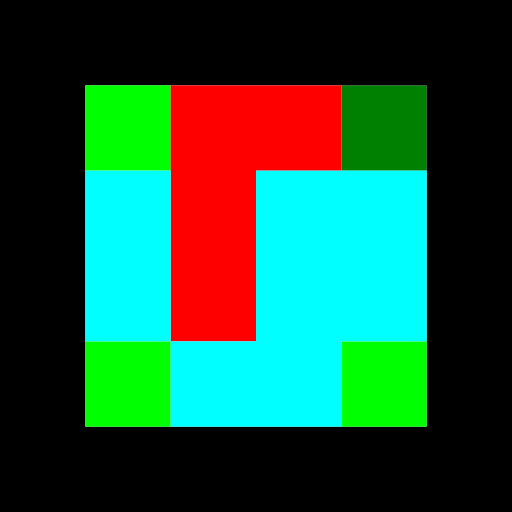
\includegraphics[width=4cm]{img/marker_template.png}
	\caption[Template Marker.]{A color coded representation of a legitimate marker. A real marker is monochrome, the colors here show the location of interesting bits. Green denotes the bits used to determine the rotation: the dark green bit is black, the rest white. Light blue denotes the binary encoded identification number of the marker. Red represents the Hamming encoded parity bits used for error correction.}
	\label{fig:marker_template}
\end{figure}

Thus encoded, the framework can by default detect 256 different markers.
This was deemed sufficient, considering the penalty in performance for each additional detected marker when running on a mobile device, as Imagine becomes unusably slow long before reaching this limit – as seen in section \ref{performance}.

\section{Usage}

Concerning the placement and creation of the marker a few points should be considered.
First off, the framework offers a helper method for creating a binary representation of a marker given an identification number.
This removes any need for the user to manually create and encode a marker and the resulting marker is guaranteed to be correct.

Secondly, the marker should be black on white, with the black border contrasted by white space around it.
Correct detection of the presence of a marker can not be guaranteed otherwise.
Generally speaking, the framework is sensitive to the contrast range of the recorded camera feed, and thus it should be maximized.
Apart from monochrome markers, this also means that the environment should be brightly and constantly lit.

Thirdly, the marker should be created and printed digitally.
The correct detection of the border is the first and most important step in the detection of the marker and should thus be as good as can be managed.
Drawing the markers by hand is possible, but will result in a loss of accuracy due to imperfections that are bound to arise with hand-drawn markers.
Care should especially be taken concerning the outermost border of the marker, as it is the main aspect used for calculating its pose.
This is only true for the border, however: the internal four by four grid containing the orientation and identification of the marker can be drawn in, so long as the drawing is done carefully.

Markers that are not smooth or have other imperfections will either outright fail in being identified or have an incorrect pose assigned to them.

% Application work:
\chapter{Application}
\subsection{Application Context}

The app is to be developed to provide a proof-of-concept for the framework.
Basic tasks of the app include showing off the capabilities of the framework, proving the implementation, and as an example on how to utilize the framework.

The app will be developed for Android 4 and above, although the framework will be independent from any Android version.
The app will force landscape view as it offers the more natural layout for the layout of the app.
Apart from OpenCV for the framework, the app shall have no further dependencies on further 3rd party tools.
This should ensure a clean and fast code for the application.

The app should be capable of running smoothly on a Tegra 3 processor\footnote{See: \url{http://www.nvidia.com/object/tegra-3-processor.html}.}.
The development device is the Transformer Prime, a 10'' tablet from ASUS\footnote{See: \url{http://eee.asus.com/en/transformer-prime/features}.}.
This means that the app should run smoothly on a 1.6Ghz Quadcore ARM processor rendering to a 1280 by 800 pixel screen.

\subsection{System Tasks}

In this section, we will take a look at the various tasks the final app should be capable of doing.
Note that we differentiate between required tasks (meaning tasks that should reliably and completely work for the app to be considered done) and optional tasks (tasks that might be included, depending on time and scope of their implementation).

\subsubsection*{Required Tasks}

\begin{tabulary}{\textwidth}{L || L}
View Camera & The user should, upon opening the app, be confronted with the view of the live camera feed. By default, if a marker is detected, a simple 3d coordinate marker is shown in place of an object. \\
\hline
Load Model & Load and prepare a 3d model to be viewed in the camera feed on top of the marker. Any model in a recognized format should be selectable as a file from a file browser. \\
\hline
Modify Model & This task shall allow the user to change basic properties such as rotation and scale of a loaded object.\\
\hline
Unload Model & Unload a model, returning the view to the standard 3d coordinate marker on top of the marker (if detected). Unloading a model can also be achieved by loading a new one to replace it. \\
\hline
Change Settings & Allows the user to modify the frames per second to render the output, how often to update the frame, and the visual quality of the video feed on which the marker detection is run. Should enable the app to be adapted to run on a wide variety of devices.\\
\hline
Toggle Debugging Information & If desirable, the user can toggle a debugging view to be rendered on top of the feed. This should offer detailed information on the shown view, marker detection, and any other factors. \\
\hline
Screenshot & As Android does not offer a screenshot tool by default, an option to capture the feed shall be provided. \\
\end{tabulary}

\subsubsection*{Optional Tasks}

This section represents tasks that could be added but might not be.
Any feature that does not make the final app is to be taken as a suggestion for possible future expansion.

\begin{tabulary}{\textwidth}{L || L}
Marker Definition & If possible, the user can load any recognized picture to be used as a marker beyond the default one. Certain properties will most likely be required of the picture however. \\
\hline
Modify Model & Further options such as toggling the rendering of a wireframe or textures. Future work might even include shader control or blending options for transparency or blur.\\
\hline
Multiple Tracker Support & Enable the app to track multiple markers at once and render their objects simultaneously.\\
\hline
Primitive Objects & Allow basic text or pictures to be used directly as an object without having to build them manually in a 3d modeling program. This feature would enable fast prototyping for text- and picture-based AR.\\
\end{tabulary}

\subsection{Dialog Structure}

Figure \ref{fig:dialog_structure} shows a graph of the usage flow in the app graphical user interface.
Note that apart from the layout change from just the main screen to the screen with the menu displayed at the right border, all sub-menus are displayed in-place to the original menu.
This allows the main purpose of the app, namely the rendering of AR, to always be in the focus of the user.
This enables rapid and direct feedback to any changes the user does within the menus.

\begin{figure}
	\centering
	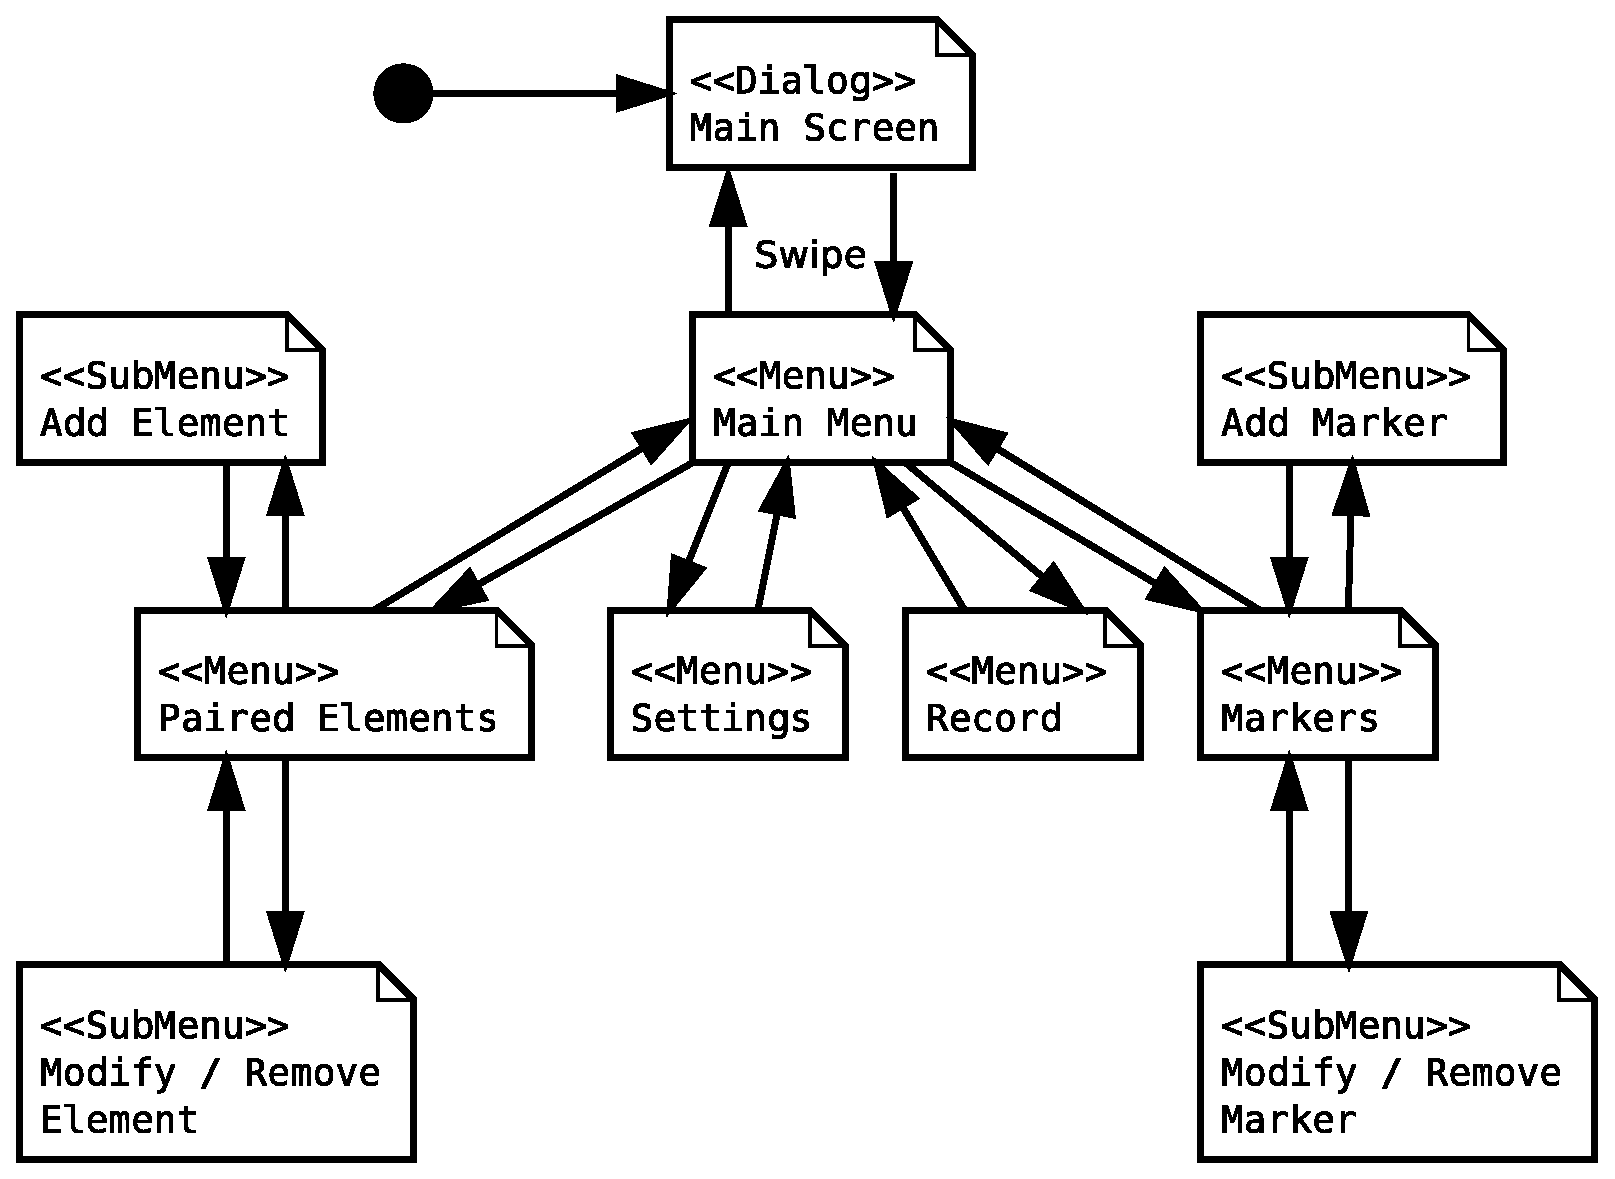
\includegraphics[width=10cm]{images/dialogs.eps}
	\caption[App Dialog Structure.]{Overview of the dialog structure of the app. Except where otherwise noted, all actions from one dialog to another are a simple touch.}
	\label{fig:dialog_structure}
\end{figure}

\subsection{Mockups}

\begin{figure}
	\centering
	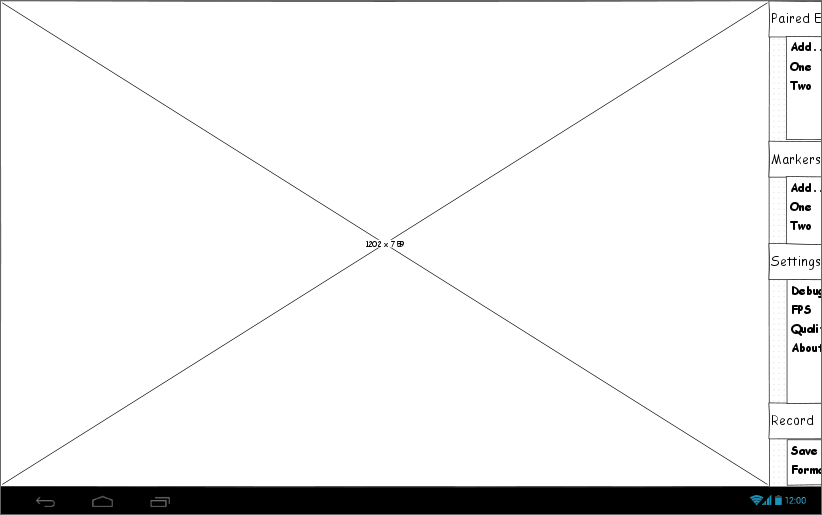
\includegraphics[width=15cm]{images/main_nomenu.png}
	\caption[Start screen mockup.]{Mockup of how the start screen of the final app might look. Note the menu partially hidden to the right, the rendered axes, and the green status light signifying that the marker is being read with a high confidence.}
	\label{fig:main_nomenu}
\end{figure}

Upon starting the app on a capable device, the app presents itself as shown in Figure \ref{fig:main_nomenu}.
This is effectively the start screen from where all the interaction takes place.

The green light in the top left shows that the app is detecting the marker with a high confidence, meaning that there are no large uncertainties.
If the marker is too warped or partially covered, the light switches to red.
If the app can still detect the marker but is having difficulties, the light switches to orange.
This mechanism is meant to offer fast and accurate feedback to the detection capability.
Another method of direct feedback is the already displayed axis-object.
This is meant to offer fast feedback to the orientation and scaling of the coordinate space to the user before a custom object is displayed.
The visibility of the axis-object can be toggled in the settings.

The menu on the right can be swiped in to be fully displayed.
The four main points are <Paired Elements>, <Markers>, <Settings>, and <Record>.

TODO: Add mockup.

<Paired Elements> lists the current paired marker-object pairs that the app can detect.
From here, the user can modify existing pairs by touching them, which opens a new menu in place with options pertaining to that pair, including its removal.
Adding new pairs is done via the <Add> button at the top, displaying a menu to select the marker and object to pair.

TODO: Add mockup.

<Markers> lists the available markers and provides options for organizing them.
Again, touching a marker opens an in-place menu with options.
Adding new markers, either by loading a picture, using a default, or taking a picture from the camera, can be done via the <Add> button.

TODO: Add mockup.

<Settings> is just that.
Here, the user can change app-specific settings such as video resolution, directories, debugging information, and more.

TODO: Add mockup.

<Record> allows the user to record the current rendering, either as a picture or possibly as a video.
The options beneath this item are for controlling those features.
% Results
\chapter{Results}
This section provides a commentary of the implementation work of the framework.
We will also take a closer look at the performance of the finished framework and where improvements can be made in the future.
To allow our work to be put into perspective, we will also compare the framework with the Aruco framework.
For that we implemented a basic application that implements the functionality of Imagine.

\section{Implementation}
\label{implementation}

Here we will take a look at the process of implementing Imagine.
First we will discuss difficulties and hardships endured during actual coding.
Then we will take a closer look at the performance of the completed framework.

\subsection{Encountered Difficulties}

% Sparse help
The first major difficulty we encountered upon beginning the implementation was the user generated documentation of the Java OpenCV for Android framework in the form of questions and answers or tutorials.
The probable cause for this is most likely due to the fact that OpenCV was originally written for desktop applications using C++.
That means that there are two major differences between the more widely used and documented version of the framework compared to the version used for this project.
The first is that one of the goals of our work was to write a Java framework, thus encouraging that we use the Java wrapper for OpenCV – therefore making the majority of C++ resources moot and hard to use.
The second difference is due to the fact that our framework's platform was to be Android, for which a few small differences existed compared to the normal use of OpenCV – such as the use of OpenCV via the elegant solution of a separate application, the OpenCV manager.
These two differences seem to have been sufficient in decreasing the usage of the Java port of OpenCV enough that documentation and accessible tutorials and examples proved to be far in between.
This forced development to rely all too often on examples written for other platforms and programming languages.
Luckily however the framework syntax is consistent, although the used data types are not always transferable.
Thus such translation work was possible but difficult.

% Lacking documentation
But not only unofficial documentation is lacking: official documentation in the form of documentation for the application programming interface and official tutorials are, for all intents, almost non existent at the time of this paper.
Comparably to the lacking user generated documentation, this can be mitigated by using material intended for C++.
C++ documentation is also all there is for the Javadoc used within the IDE.
It is not easy working in Java with C++ code as Javadoc, with further text mostly not relevant to the problems encountered when coding with it.

% Problems with stupid mat
While we're on the topic of the C++ base of OpenCV, allow us to criticize the single most frustrating aspect of using OpenCV: the matrix object data type, short mat.
Mats are used within OpenCV as a one-size-fits-all solution for any data ranging from vector points that represent polygons to multi-channel images in various more or less used formats.
While it was still easy to recognize the RGBA format\footnote{RGBA stands for, respectively: red, green, blue, alpha. This depicts the order and type of channels for an image.} that the framework receives the camera image in, using the correct conversions and the correct mat subtypes in the principle work thread within Imagine proved to be very frustrating.
First we encountered difficulties with the conversion of different image formats to other formats, an operation that costs a good bit of processing power and time.
Thankfully, we were able to work around any conversions by parallel usage of multiple mats whose results are used on one another to retain a higher overall speed.

Then another difficulty emerged while using the OpenCV function to calculate polygons for detected contours within an image.
The method for these polygons returns these in a special mat subtype that is specialized for floating point numbers.
However, the methods we then required to work with these polygons required the polygons in a normal mat, thus forcing us to convert from one type of mat to another.
Again this problem could largely be mitigated by converting as little as possible, although the base conversion proved to be one of the smaller problems in the overall context of speed within the Imagine worker threads.
Furthermore, there exist no methods for determining the type and allocation of channels within a mat.
While not being able to check for these properties forced a clean usage of the data class within Imagine and thus probably increased speed somewhat, such methods are crucial for learning the correct usage of mat and certainty of stored data type.
Writing and reading data with mats is also something that requires faith, as no checks for sanity can be performed on the data.
For example, the method for reading a single coordinate returns a double array – always, even when using the mat for binary images (in which case a boolean would suffice), luminance images (possibly a short data type), or as an integer matrix (integers).
The returned value then has to be cast to the (hopefully) correct data type – and if we made a mistake somewhere along the line and the mat doesn't contain the data we expect it to contain, we have no tools that would help us catch that mistake.
We therefore kindly suggest that OpenCV for Android make use of the Java generics mechanism, as we believe that would start to reduce the confusion surrounding mats.

% Problems debugging
A further difficulty proved to be the debugging of errors while programming the worker threads within Imagine.
This came from the fact that OpenCV runs in C++ even on Android and tracing errors to their source thus proved difficult.
Often only careful consideration of error messages and stack traces in the depths of the Android log allowed any progress to be made in tracing a bug, although mostly trial and error proved to be the primary method of correcting these errors.
Problems debugging errors were also due to the paradigm differences in error handling between how Java in general does it (using so-called exceptions) and C++ does it (using integers as error codes).
OpenCV for Android does not cast the numeric error codes into equivalent Java exceptions, instead leaving them as-is.
Furthermore, the numerical error codes proved to be very generic in their implications.
An example of this can be found with the error code we mostly fought with, which was 215.
That numerical error can (and does!) mean anything from incorrect mat sizes to incorrect number of channels.
A quick search also showed that the very same code is also used to signal unimplemented methods within OpenCV itself.

% Paradigm problems
While on the topic of paradigm differences: another difficulty we encountered with OpenCV for Android was the difference in coding styles.
With this we mean for example that the result of a method was not returned, but instead called by reference\footnote{This stems from the way C++ usually does error handling by returning numerical error codes. The result is written into a referenced data class, freeing the return call for passing back numerically coded error or success messages.}.
Due to the existence of exceptions, this is usually done differently when using Java.
While generally more of a nuisance than a source of error, it would be helpful if the wrapper took care of the paradigm shift between Java and the C++ interface, thus freeing developers from having to work with two paradigms in parallel.

% General
Generally speaking, OpenCV for Android proved usable for this work, but with some difficulty, as can be seen by the lengthy dissection here.
OpenGL ES proved to relatively trivial to use, notably because of the wealthy online resources in the form of extensive documentation and multiple tutorials.
The only bigger difficulties encountered while working with OpenGL ES were using multidimensional math for the matrix operations and how to get the renderer to render to a transparent layer.

\subsection{Performance}
\label{performance}

Here, we will take a brief look at the general performance of the Imagine framework.
All numbers that will be given are approximations only, as we did not statistically analyze them.
For a more in depth look of Imagine's performance, further work can be done as necessary.

\subsubsection{Frames per Second}

To give the following numbers a frame of reference, here some numbers concerning the general speed of the Android platform, and the OpenGL ES and OpenCV utilization on it.

OpenCV captures the preview frame of the camera from Android for the base frame from which all processing originates.
This means that the speed at which it does this is the first important reference for all further values.
The speed of this operation proves to be the first limiting factor: due to how Android camera capture works, the preview only offers 15 frames per second.
This was measured by simply showing the image as received through OpenCV, meaning that there was no overhead work being done.
This has some strong implications for the Imagine framework: however much the work done can be optimized, it will never be capable of running faster than that.
As humans only begin to see a smooth video upwards of approximately 20 frames per second – for perfectly smooth video however at least 60 frames per second – this places Imagine already outside the range of smooth output.

Android itself renders the interface at 60 frames per second\footnote{As of Android 4.1.}.
OpenGL ES also easily achieves 60 frames per second, although it is to note that the graphic pipeline has the advantage of serious hardware acceleration.
Of course the speed at which OpenGL ES will render a scene for the Imagine framework is highly dependent on the complexity of the models, although that should not be a limiting factor for some time yet.

The comparison of these two limiting factors shows that Imagine is mainly performance dependent on the OpenCV for Android framework.
Newer versions of it should theoretically be able to increase the speed up to the framerate of the camera preview.
To achieve even higher speeds, the speed at which Android fetches the camera preview must be increased, which could happen with newer devices and or newer version of Android.
All of these possible speed increases however lie outside of the influence of the Imagine framework.

\begin{figure}[H]
	\centering
	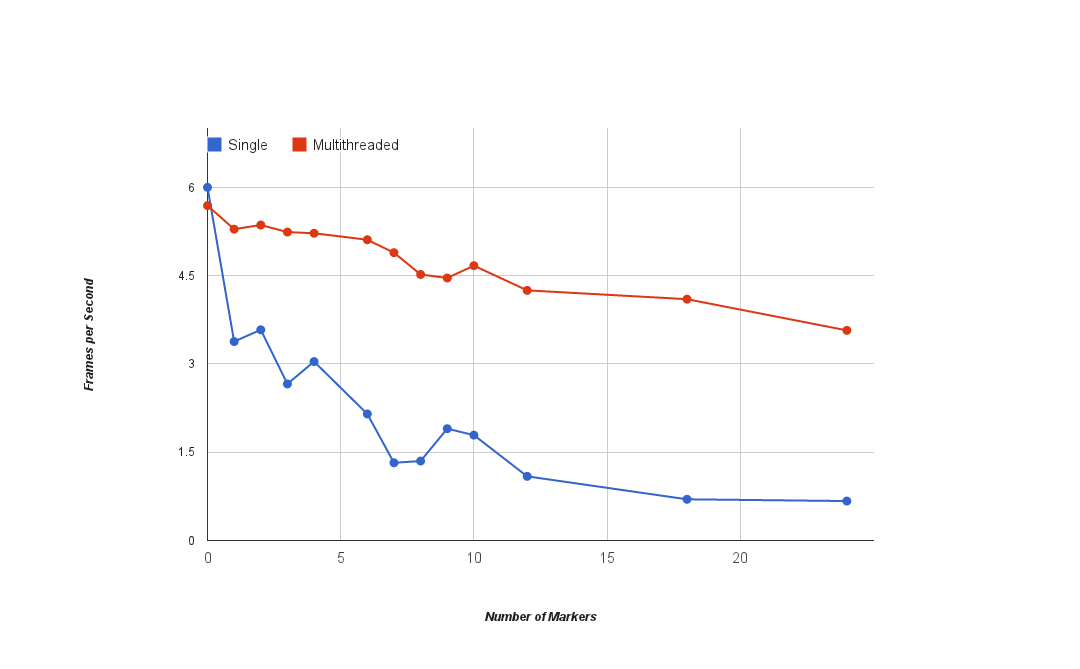
\includegraphics[width=16cm]{img/performance_chart.png}
	\caption[Imagine Performance Chart.]{This chart shows the performance in frames per second of Imagine, working both as a single pipeline and with multithreading.}
	\label{fig:performance_chart}
\end{figure}

For the speed of the Imagine framework, a general understanding of the algorithm that detects markers is required – as can be found in section \ref{detection_workflow}.
Imagine idles at up to \textbf{seven frames per second}, meaning that this is the best case performance under ideal circumstances with no markers present.
When markers are present and detected, performance takes a hard dip.
This and the difference multithreading makes can be seen in figure \ref{fig:performance_chart}.

\subsubsection{Speed of Operations in Detector}

The first performance sensitive operation is the \textbf{conversion of the input image into a binary image}.
The default method with a static threshold takes around 8 ms.
It is significantly faster than adaptive thresholding with 88 ms.
However it does not work reliably in low contrast images or in high dynamic ranges within an image.

Next is the \textbf{operation that finds all contours from the binary image}.
This operation is a vital part of the algorithm and can not easily be exchanged for some other operation.
The cost of finding contours varies strongly on the binary image, but generally takes around 22 ms.

Now Imagine has to \textbf{process each contour separately}, as each could be a marker.
This step is where most of the performance is siphoned from.
In total these operations take around 100 ms, with a high variance for the number of markers.

For each found contour, we \textbf{calculate the polynomial approximation} and use it to filter out any polygons that aren't convex and don't have 4 corners.
This step takes about 3 ms.
Imagine then calculates the perspective transform and applies it to \textbf{dewarp the texture} of the marker candidate to allow sampling.
Using the RGBA input mat, OpenCV does this step in 12 ms.
Originally however we require a grayscale image at this point; however it turns out that OpenCV has no hardware acceleration for dewarping grayscale mats on a Tegra CPU, such as the developer machine has.
Using the grayscale image would impose a more hefty performance cost.

If the contour is still a valid candidate at this point, Imagine tries to \textbf{detect a marker} from it and the dewarped texture.
This method takes anywhere from 5 ms to 30 ms, depending on whether the candidate is valid in terms of sampling its properties from the texture (meaning valid border, orientation, and identification marks).
If a marker is rotated, then the correction of the identification pattern takes additional time, as rotating matrices is computationally expensive.

Now only one step remains for a complete marker detection: \textbf{calculating the perspective transformations}.
This is done for all detected markers, but luckily is relatively fast compared to other operations.
OpenCV takes 2 ms to calculate the data for every marker.

\section{Features and Capabilities}

In this section, we will take a look at the implemented features of Imagine.
This includes basic features that are required for basic usability and capabilities for debugging various algorithm stages.

\subsection{Debugging Capabilities}

Imagine offers some easy options for selective debugging beyond the log output on Android.
Specifically for debugging the visual pipeline we implemented some options so that pinpointing an error is comparatively easy.
Setting debugging up is done via flags and should only be done before calling the onCreate method.

The first option we offer is to \textit{activate a more verbose logging mode}, where Imagine logs quite a bit more information concerning possible errors – for example, the status of the hamming decoding upon marker detection.
On par with that one can also \textit{activate frame per frame time logging}, where Imagine will log the time each detection and rendering step takes.

Going into the visual debugging it is important to note that marker detection is partially suspended.
In any case Imagine deactivates multithreading to enable the output to be shown – as seen in section \ref{performance}, this decreases performance quite a bit.
Once in visual debugging mode, three main aspects can be shown.
The first option that can be activated \textit{shows the binary picture}.
This can be used to check whether the chosen binarization method is working correctly.

Another output that can be chosen is to let Imagine \textit{draw the detected contours}.
This option can be used to detect errors within the contour detection that arise from the method used to binarize the image.

\begin{figure}
	\centering
	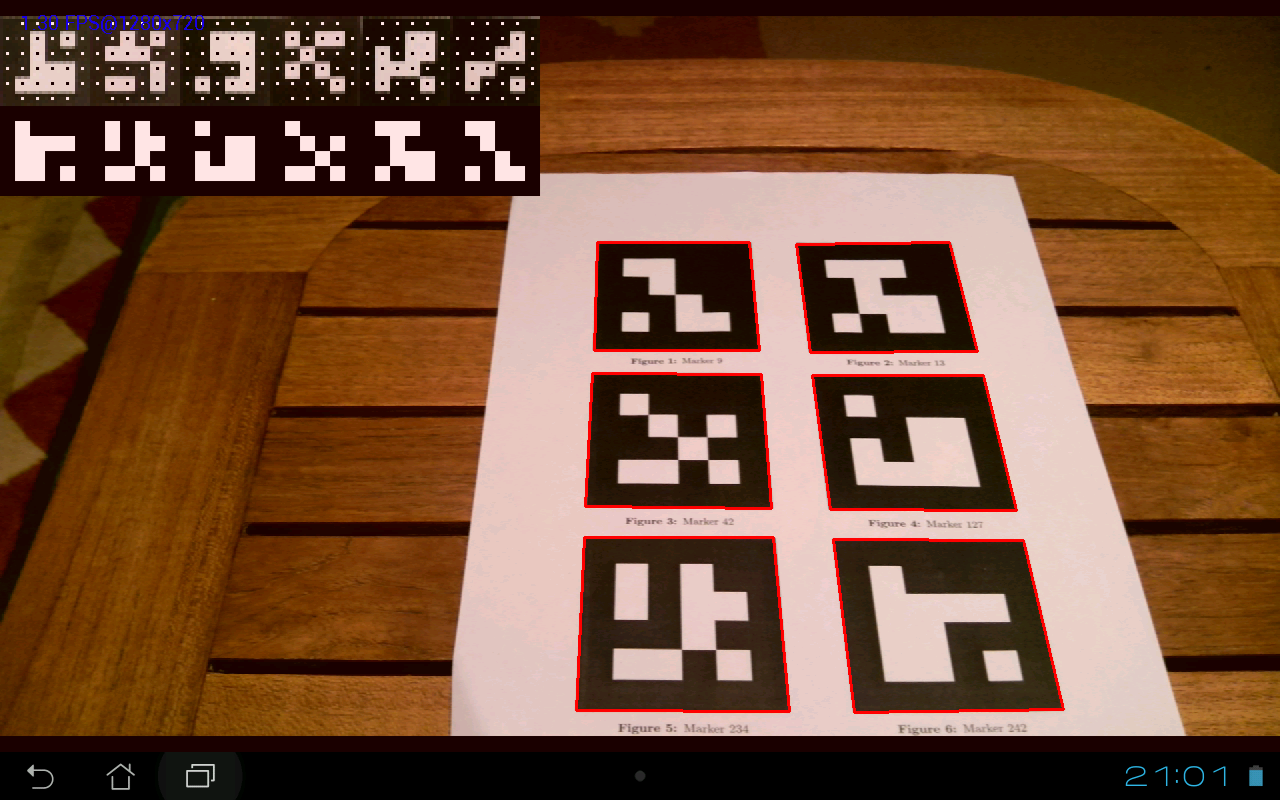
\includegraphics[width=10cm]{img/debugging_view.png}
	\caption[Debugging View]{A screenshot of how the three more relevant debugging views can look. Shown are the polygonal rendering (perspective red squares around markers), the marker texture with the sampling points, and the correctly rotated processed marker pattern.}
	\label{fig:debugging_view}
\end{figure}

The following visual debugging methods are the more helpful ones.
Figure \ref{fig:debugging_view} shows how the polygonal rendering, the texture sampling of markers, and the detected identification pattern are shown.

Of these, the option to display the polygons of detected markers is best used to check that Imagine sees a marker.
Here, Imagine draws the perspective bounding box of all marker candidates that have been detected.
To check whether Imagine correctly samples a marker candidate, both the option to draw the marker textures and the marker identification patterns can be used.
Drawing marker textures can verify that Imagine has correctly dewarped a texture and show how warped the marker surface was.
This can be seen when the dewarped marker texture is not perfectly aligned with the square sampling.
The marker identifications can be used in conjunction with the option to draw the sampling onto the marker textures to check whether Imagine is correctly sampling the pattern of candidate markers.

All of these debugging capabilities arose out of the step-by-step development process.
Once we realized how useful such functions were, we decided to keep them accessible from the outside.
Thus we made sure that they work relatively well and can be activated easily\footnote{This is realized by the methods in MainInterface for setting and removing debugging flags.}.

\subsection{Features}

Of the features listed in section \ref{scope_limit}, the following are accessible and usable.
Debug messaging is possible beyond the functionality already offered by Android, most notably a unified logging mechanism and timing functions.
Managing so-called trackables is possible, including the on-the-fly adding, removing, and exchanging of marker-object associations.
Reading the pure 3D transformation data is also possible via a listener, bypassing the graphical part of Imagine.
Manual configuration is somewhat possible, as many values can be changed to accomondate special use cases.
It is however easily possible to configure debugging views to display relevant information and to enable extensive debugging output.
Multithreading is also implemented and beneficial, as seen in section \ref{performance}.
If required or when debugging views are to be used, a single thread pipeline can also be used.

Therefore we conclude that our framework covers the basics in functionality, although a multitude of improvements can be made.
These improvements are listed in section \ref{improvements}.

\section{Application}

To enable rapid testing and experimenting, we implemented a basic application for evaluating our framework.
It consists of two activities: one for setting parameters and control values and one for actually running the framework.

Figure \ref{fig:debugging_view} is a screenshot of the application running the framework activity with debugging values activated.

TAMINO TODO: TODO AND MORE!

\section{Comparison to similar Apps}

In this section, we will compare Imagine to two other marker-based augmented reality frameworks for Android.
Both are open source projects and can be used freely in personal projects.
Table \ref{comp} lists the main differences.

\begin{table}[H]
	\centering
	\begin{tabulary}{\textwidth}{J | J | J | J}
	\textbf{Framework} & \textbf{FPS} & \textbf{Number of markers} & \textbf{Maximum parallel markers} \\
	\hline
	Imagine & ~5 & 256 & 256 \\
	\hline
	Aruco & ~4 & 1024 & unknown \\
	\hline
	DroidAR & unknown & 4096 & 5 \\
	\end{tabulary}
	\caption[Performance Comparison]{Short table of feature comparison of Imagine, Aruco, and DroidAR.}
	\label{comp}
\end{table}

\subsection{Aruco}

Aruco \cite{aruco} is a minimal library for Augmented Reality applications based on OpenCV.
Primarily, it is intended for desktop C++ applications, although an Android port and web-based Javascript port exist.
For the purpose of comparing it to our own framework, we will base the comparison on the Javascript port \cite{jsaruco} running on the same developer machine.

\begin{figure}[H]
	\centering
	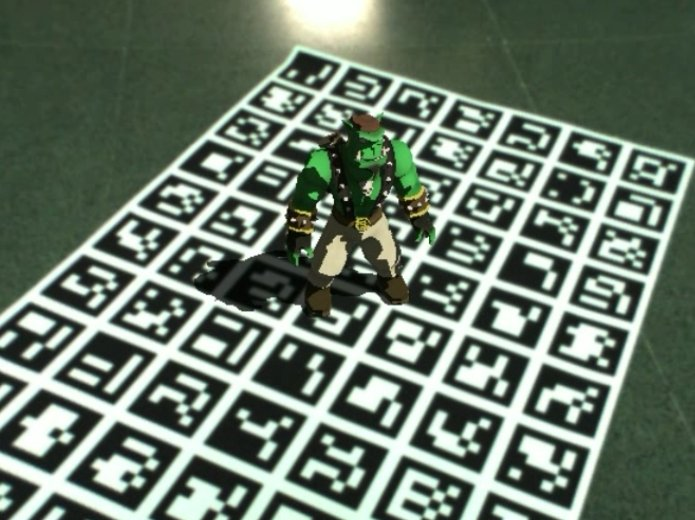
\includegraphics[width=8cm]{img/aruco.png}
	\caption[Aruco]{Screenshot of a basic Aruco application.}
	\label{fig:aruco}
\end{figure}

The main features of Aruco are simple usage, 1024 markers that can be identified, and the support of so-called AR boards\footnote{Markers composed of several markers for higher reliability.}.
The marker detection algorithm used by Aruco is the basis for our own work and thus works similarly.
The main differences in implementation are that Aruco does sub pixel accuracy and a higher number of markers.
These are advantages of Aruco over Imagine.

The Javascript port runs at around four frames per second in a mobile web browser.
This is a low difference compared to Imagine, although our framework runs natively.
We believe this due to the fact that while Aruco is based on OpenCV, the Javascript port can not use the library, and thus re-implements the required features.
That removes any overhead caused by unused features and allows a completely native environment for data objects, without any significant conversions having to be done, which were one bottleneck in Imagine.
Nonetheless Imagine is a small step faster.

\subsection{DroidAR}

DroidAR\cite{droidar} is another framework for Android that allows, among other Augmented Reality features, marker-based tracking.
Due to difficulties using the framework on the developer's machine, no performance comparison could be made.
DroidAR could not be tested solely without any other features without writing an application for that, which is beyond the scope of this comparison.

\begin{figure}[H]
	\centering
	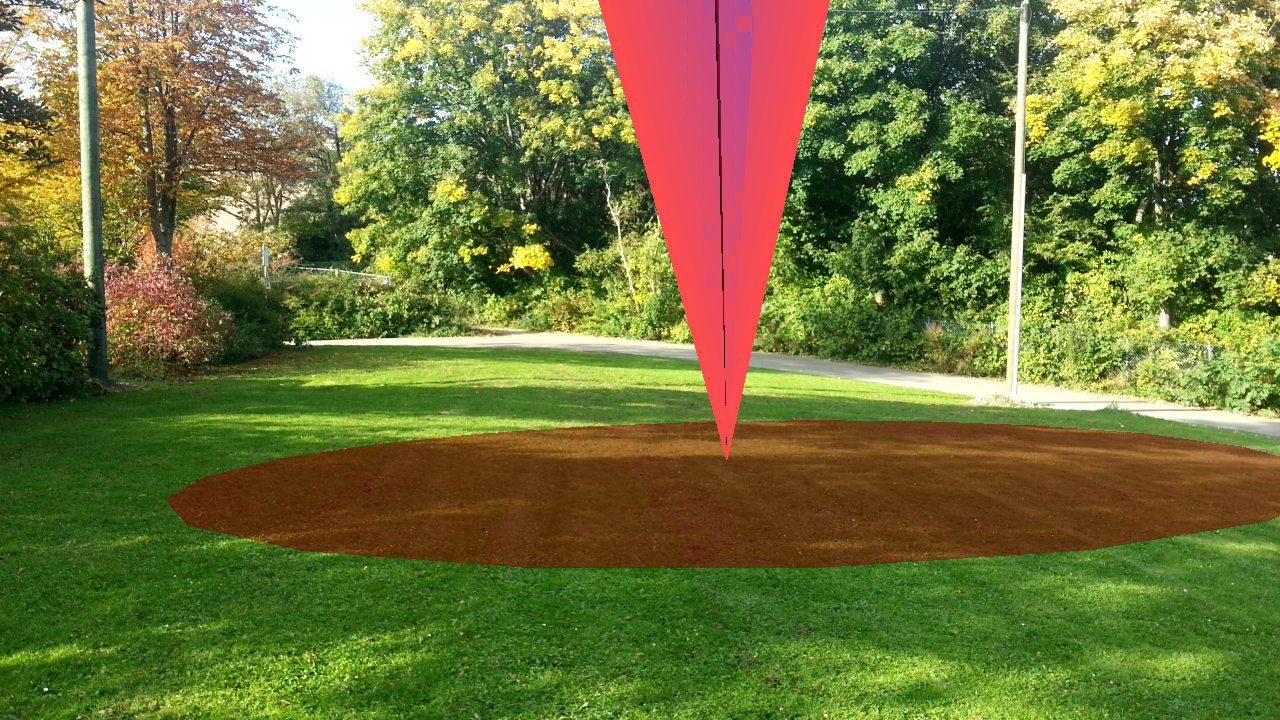
\includegraphics[width=10cm]{img/droidar.png}
	\caption[DroidAR]{Screenshot of a basic DroidAR application.}
	\label{fig:aruco}
\end{figure}

Feature wise a few things are different compared to Imagine, although some interesting parallels also exist.
Most notably, DroidAR uses threads for the detection of markers and also utilizes OpenCV for Android.
The detection method is also similar to both Aruco and Imagine.
However, the actual detection is done with native C++ code.
DroidAR can differentiate 4096 markers, although only 5 can be detected at once, probably for performance reasons.
Imagine can detect more than 5 markers in parallel, DroidAR however has a faster implementation.

% Conclusion
\chapter{Conclusion}
Finally we will give a broad overview of the accomplishments of this work, difficulties encountered, possible improvements, and use cases.
We will finish with a broad closing statement.

\section{Future Possibilities}
\label{future}

While basically completely usable, there are many aspects that can still be improved.
These range from performance considerations, porting Imagine to other platforms, to extending the functionality offered.
In this section, we will propose some aspects that we think could be of interest for future work as they were beyond the time scope of this project.

\subsection{Performance}

Concerning the performance of Imagine a lot could still be done, although globally the performance will remain limited by the capabilities of OpenCV for Android.
One of the main aspects that could be tried however is writing the main method that detects markers using OpenCV with native C++ and calling that from the Java environment with a native call.
We did not try that because of two factors: one, a basic Java framework was the primary goal, and two, developing a Java application for Android with native code in C++ would have put this work beyond our time frame.
It would also have further divided our attention away from the core functionality, as considerable time would have had to be spent learning and utilizing the native development kit.

We are also confident that some aspects of the OpenCV code could be optimized even further, although that might require a more significant analysis with better and robuster timing features.
The performance of the worker threads when using multithreading could certainly also be improved further, as multithreading is hard to do correctly.

Apart from Imagine, improvements in the runtime environment – Android itself – could yield further speed gains, although that would most definitely be beyond the scope of the framework and take a lot of time.

Apart from software aspects various hardware considerations could also lead to better performance.
One would be the increase of the speed at which the camera generates preview images, allowing OpenCV to grab these faster for further accessing.
A higher count of CPU cores could also serve to increase the speed by running more worker threads.
A faster CPU than the 1.4 Ghz quadcore used here will should also increase performance.

\subsection{Features}

While Imagine offers a basic rendering system, it lacks a decent rendering system for production use that can fully utilize the OpenGL ES 2.0 framework.
Shading, texturing, and animation would benefit the use-cases greatly.
These features however would be a project unto itself and was thus left for a future time.

Another feature that would make using Imagine easier is implementing either a lookup model for camera values or offering an internal method for generating them.
This would allow the removal of determining these numbers externally into the framework, further abstracting away possible hurdles to using it.

To improve resistance against marker occlusion and increase marker detection precision, support for marker boards such as used by Aruco could also be added.
However we believe that implementation of such a capability would only be feasible once Imagine has better performance, as the number of markers required for a marker board greatly decrease the framerate.

\subsection{Improvements}
\label{improvements}

From an architectural standpoint, the flow of data within the framework could be improved.
Especially the transfer of data to and from the worker threads could surely be solved better to remove execution blocks.
Most notably the fetching of input frames could be resolved so that the live preview drawn in the background were independent in speed from the worker threads.
This would however require extensive knowledge of multi-threading, and was thus deemed beyond the scope of this project.

The external application programming interface could be expanded too to allow a better and more detailed control of the inner workings.
Care should be taken to keep the basic simplicity of using the framework though.
Internal states that could be opened to external control include the resolution of the images, rendering settings, and marker properties.

Internally, Imagine could be expanded to refine corners using subpixel interpolation when detecting the contours of possible markers.
The OpenCV method for subpixel precision is however expensive in terms of performance.
The advantage of subpixel interpolation would be a better pose estimation, removing sudden jumps and improving the visual fidelity.

\subsection{Extended Possibilities}

Speaking on a more general view, some extended possibilities for future work offers themselves.
One of the more interesting ones would be the porting of the framework to other platforms, most likely for desktop computers first as they offer significantly more processing power.
Higher graphical fidelity and more features for the rendering side would also become a possibility.

A further possibility would be the harnessing of further OpenCV functionality concerning the adaptability of the output.
This could range from situation aware rendering concerning the lighting of models to detection of further information from objects found in the scene.

\section{Closing Statement}

We have shown our results of implementing a Java framework for Android for marker based detection to be used in augmented reality programs.
This includes preparatory work for the framework and the basic application that utilizes it, to the finished results.
The framework, called Imagine, covers the basic required features to be fully functioning, although various aspects could still be greatly improved and expanded upon.

Apart from the framework, documentation and explanation of its workings have been created.
Documentation is to be found in the Javadoc of the project, also seamlessly accessible by any modern IDE during active development.
This paper highlights the internal functionality of Imagine and how to access it.
Insight into debugging capabilities and possible areas where difficulties might arise are also highlighted.

We have also shown some possibilities for further work that would significantly expand the use-cases of our framework.
To help with future evaluations we have also done some basic benchmarks and timed the currently most processing intensive part – the detection algorithm.

All in all, we are satisfied with the promise of Imagine, although in detail there are many areas worthy of more development time.
We consider the framework to be academically usable, but would refrain from utilizing it in a production scenario due to low performance while detecting markers.
We believe the code of Imagine however to be an excellent starting point to learn how to implement augmented reality applications as it provides at the very least a basically functional framework.

%Glossary
\chapter*{Glossary}
This section provides a brief overview of the used terms in the paper and what they mean as we understand.
We make no claim for completeness or correctness.

\begin{tabulary}{\textwidth}{L|L}
Augmented Reality & Refers to a live, direct view of a physical, real-world environment whose elements are augmented by computer-generated sensory input\protect \cite{ardef}. \\
\hline
Trackable & The object used by Imagine to combine detected marker information with data to be used when rendering. Not externally accessible.\\
\hline
Entity & The user created object used by Imagine to register a marker to track, complete with 3d model information to be shown when the corresponding marker is detected. Externally accessible.\\
\hline
Marker & A printed or displayed significant pattern which the system can recognize through image detection. Used to represent the location of the augmented space projected by the system. \\
\end{tabulary}

Android, 3D, Imagine, OpenCV for Android, OpenGL ES, Java, IDE, de-warp, activity, 


\appendix
%\input{sources}

\backmatter

\listoffigures
% TODO: Get this to work without making all my tables float away... :P
%\listoftables

% Bibliograhpy
\bibliographystyle{alpha}
{\small
\bibliography{literature.bib}
}

\clearpage
\erklaerung

\end{document}
